\subsection*{A1 --- Complete overall metrics (Objective 1)}
\begin{table}[h]
\centering\scriptsize
\caption{A1. Pooled out-of-fold scores, 50 training groups, with 95\% pool-bootstrap intervals.}
\label{tab:A1}
\resizebox{\linewidth}{!}{
\begin{tabular}{llcccc}
\toprule
 & Predictor & NLL & Brier & AUROC $\times100$ & ECE $\times100$ \\
\midrule
Llama & Structure only & 0.5035 [0.4310, 0.5849] & 0.1392 [0.1236, 0.1548] & 69.5 [65.5, 73.4] & 6.70 [5.12, 8.47] \\
Llama & B1 & 0.4820 [0.4116, 0.5599] & 0.1347 [0.1190, 0.1502] & 71.5 [67.2, 75.8] & 6.50 [4.98, 8.24] \\
Llama & B2 & 0.4013 [0.3497, 0.4548] & 0.1153 [0.1005, 0.1302] & 78.9 [75.5, 82.2] & 4.58 [3.19, 6.24] \\
Llama & H1+S & 0.4138 [0.3618, 0.4692] & 0.1176 [0.1039, 0.1315] & 77.4 [73.6, 80.9] & 4.23 [2.97, 5.79] \\
Llama & H2+S & 0.3934 [0.3431, 0.4468] & 0.1123 [0.0984, 0.1269] & 80.2 [76.8, 83.5] & 4.44 [3.16, 6.05] \\
Llama & RCAP & 0.3897 [0.3422, 0.4409] & 0.1113 [0.0982, 0.1247] & 80.2 [76.9, 83.4] & 4.37 [3.22, 5.78] \\
Llama & B1+H1 & 0.4131 [0.3651, 0.4617] & 0.1183 [0.1043, 0.1324] & 79.0 [75.7, 82.0] & 5.39 [4.11, 6.97] \\
Llama & B2+H1 & 0.3849 [0.3380, 0.4344] & 0.1111 [0.0972, 0.1253] & 80.8 [77.5, 83.8] & 4.36 [3.03, 5.93] \\
Llama & B2+A1 & 0.3821 [0.3344, 0.4321] & 0.1096 [0.0959, 0.1235] & 81.2 [78.2, 84.1] & 4.44 [3.28, 5.91] \\
\midrule
Qwen & Structure only & 0.3560 [0.2856, 0.4334] & 0.0913 [0.0752, 0.1082] & 70.9 [65.1, 76.5] & 5.63 [4.17, 7.47] \\
Qwen & B1 & 0.3404 [0.2758, 0.4111] & 0.0885 [0.0736, 0.1042] & 72.5 [67.0, 78.0] & 5.36 [3.73, 7.11] \\
Qwen & B2 & 0.2927 [0.2402, 0.3494] & 0.0769 [0.0633, 0.0910] & 77.1 [72.2, 82.0] & 3.74 [2.49, 5.23] \\
Qwen & H1+S & 0.2822 [0.2370, 0.3311] & 0.0767 [0.0639, 0.0900] & 80.3 [76.3, 83.9] & 3.76 [2.63, 4.97] \\
Qwen & H2+S & 0.2741 [0.2292, 0.3220] & 0.0744 [0.0619, 0.0876] & 81.2 [77.1, 84.9] & 3.37 [2.25, 4.60] \\
Qwen & RCAP & 0.2741 [0.2291, 0.3230] & 0.0731 [0.0610, 0.0857] & 81.5 [77.3, 85.3] & 3.83 [2.68, 5.05] \\
Qwen & B1+H1 & 0.2880 [0.2416, 0.3379] & 0.0783 [0.0651, 0.0921] & 79.6 [75.7, 83.2] & 3.91 [2.79, 5.10] \\
Qwen & B2+H1 & 0.2741 [0.2291, 0.3219] & 0.0745 [0.0620, 0.0876] & 81.1 [77.1, 84.8] & 3.35 [2.24, 4.59] \\
Qwen & B2+A1 & 0.2734 [0.2286, 0.3221] & 0.0729 [0.0609, 0.0856] & 81.5 [77.4, 85.4] & 3.77 [2.61, 4.99] \\
\bottomrule
\end{tabular}
}
\end{table}

\begin{table}[h]
\centering\scriptsize
\caption{A1 (contrasts) and A4 (sensitivity). Brier reduction $\times10^3$; NLL reduction $t_{49}$ interval and leave-one-pool-out range (nats).}
\label{tab:A1c}
\resizebox{\linewidth}{!}{
\begin{tabular}{llccc}
\toprule
 & Comparison & Brier reduction & NLL $t_{49}$ interval & NLL leave-one-pool-out \\
\midrule
Llama & 1: B1 \cto{} H1 & 17.04 [10.56, 23.87] & [0.0341, 0.1024] & 0.0589 to 0.0709 \\
Llama & 2: B2 \cto{} H2 & 2.92 [$-$0.24, 6.11] & [$-$0.0027, 0.0185] & 0.0055 to 0.0096 \\
Llama & 3: B2 \cto{} RCAP & 4.00 [$-$0.88, 8.88] & [$-$0.0047, 0.0279] & 0.0079 to 0.0150 \\
Llama & 4: H2 \cto{} RCAP & 1.08 [$-$3.00, 5.70] & [$-$0.0122, 0.0196] & $-$0.0014 to 0.0059 \\
Llama & 5: B1 \cto{} B1+H1 & 16.40 [9.20, 23.81] & [0.0253, 0.1126] & 0.0574 to 0.0737 \\
Llama & 6: B2 \cto{} B2+H1 & 4.19 [1.71, 6.63] & [0.0071, 0.0255] & 0.0139 to 0.0179 \\
Llama & 7: B2 \cto{} B2+A1 & 5.68 [2.35, 9.62] & [0.0073, 0.0310] & 0.0160 to 0.0210 \\
\midrule
Qwen & 1: B1 \cto{} H1 & 11.80 [6.12, 17.79] & [0.0229, 0.0937] & 0.0471 to 0.0640 \\
Qwen & 2: B2 \cto{} H2 & 2.46 [$-$0.78, 5.64] & [0.0027, 0.0345] & 0.0147 to 0.0213 \\
Qwen & 3: B2 \cto{} RCAP & 3.81 [$-$0.56, 9.04] & [$-$0.0007, 0.0379] & 0.0134 to 0.0214 \\
Qwen & 4: H2 \cto{} RCAP & 1.35 [$-$2.50, 5.58] & [$-$0.0134, 0.0134] & $-$0.0030 to 0.0027 \\
Qwen & 5: B1 \cto{} B1+H1 & 10.16 [5.45, 15.27] & [0.0213, 0.0836] & 0.0422 to 0.0564 \\
Qwen & 6: B2 \cto{} B2+H1 & 2.38 [$-$0.89, 5.52] & [0.0029, 0.0343] & 0.0149 to 0.0211 \\
Qwen & 7: B2 \cto{} B2+A1 & 3.93 [$-$0.42, 9.18] & [$-$0.0002, 0.0387] & 0.0140 to 0.0220 \\
\bottomrule
\end{tabular}
}
\end{table}

\subsection*{A2 --- Calibration (Objective 1)}
\begin{figure}[h]\centering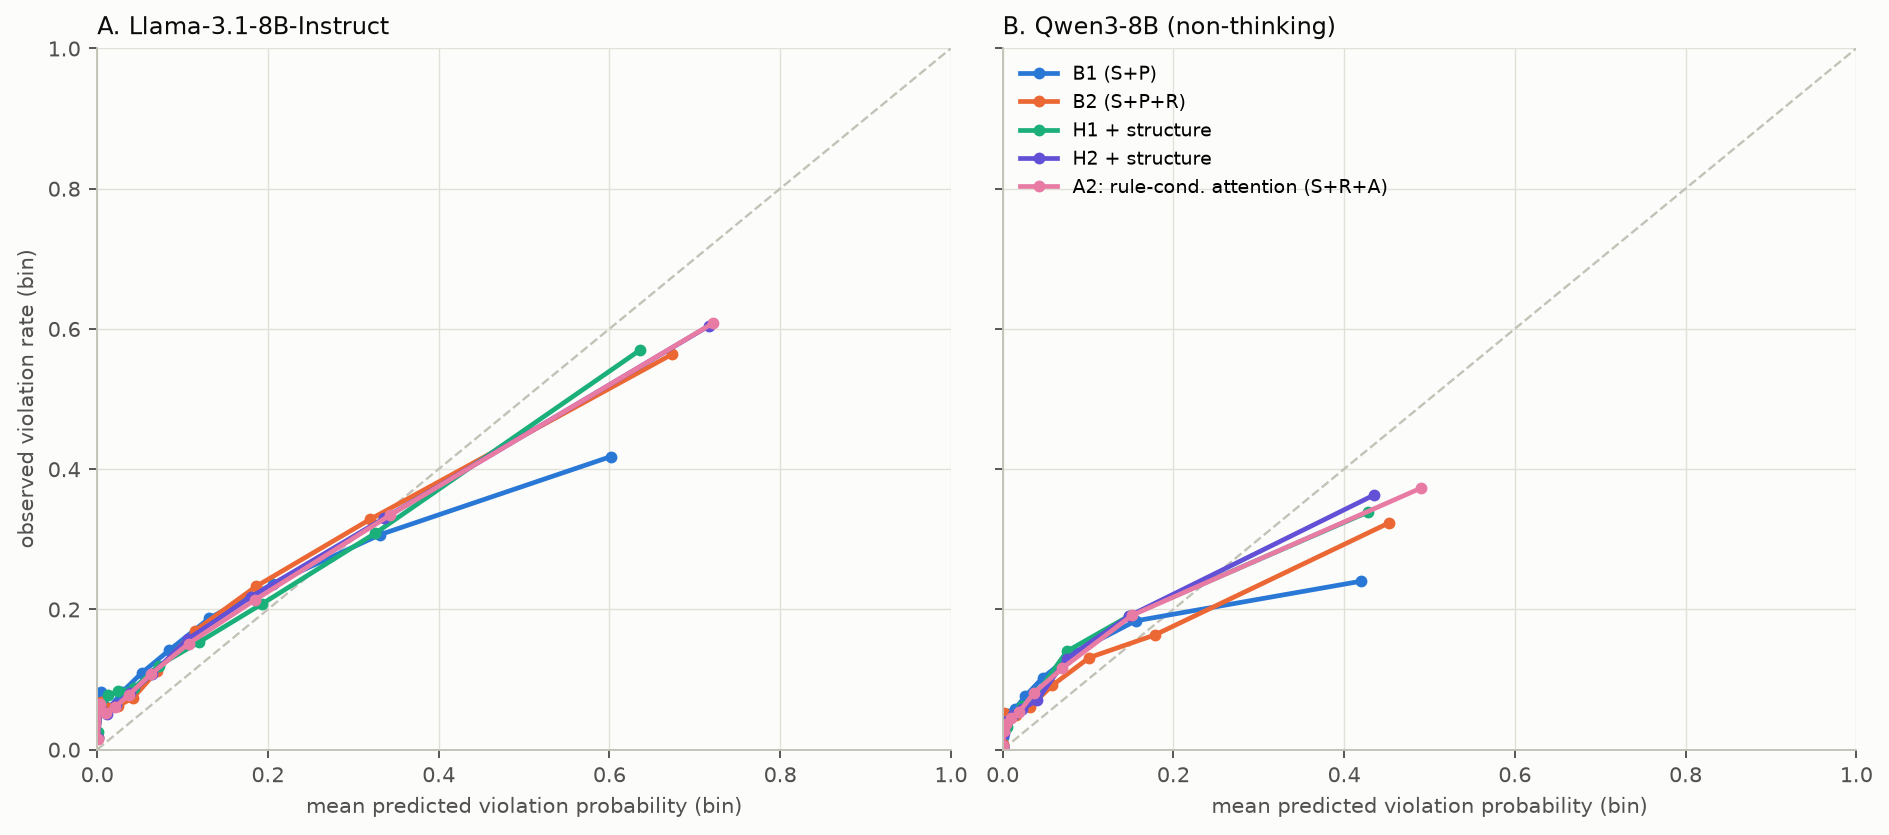
\includegraphics[width=\linewidth]{figures/prelim/e1_A2_reliability.png}\caption{A2. Reliability curves (out-of-fold, decile bins of each predictor's own predictions).}\end{figure}
\subsection*{A3 --- Per-type NLL reduction}
\begin{figure}[h]\centering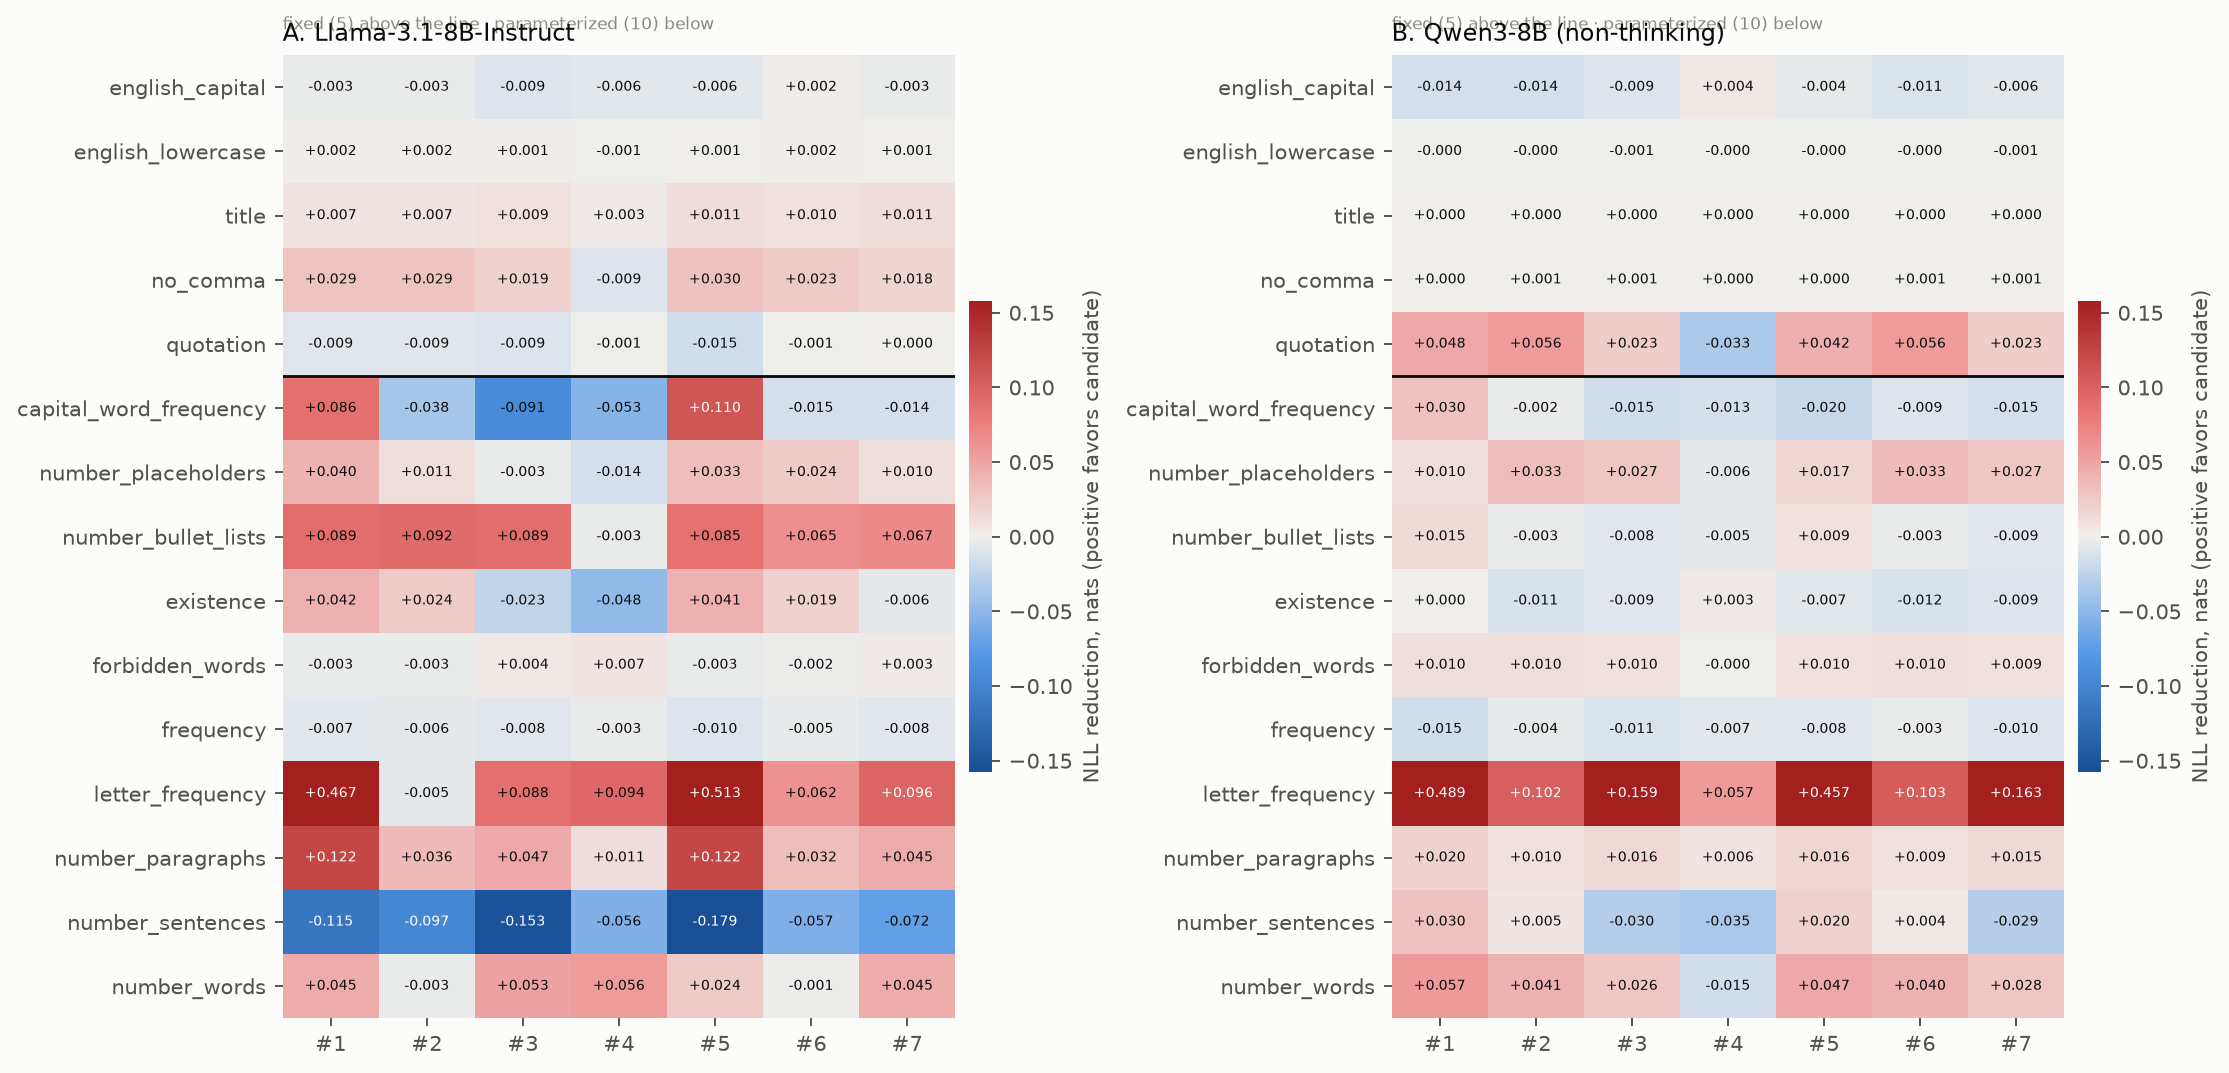
\includegraphics[width=\linewidth]{figures/prelim/e1_A3_per_type_nll_heatmap.png}\caption{A3. Per-type NLL reduction for the seven comparisons; five fixed-wording types above the line. All 210 values with paired intervals and support: \texttt{tables/eval1\_per\_type.csv}.}\end{figure}
\subsection*{A3b --- Fixed versus parameterised rule types (Objective 1 only)}
\begin{table}[h]
\centering\scriptsize
\caption{A3b. NLL reductions (nats) of the seven comparisons within the five fixed and ten parameterised types, and their difference (fixed $-$ parameterised improvement); identical 50-pool resamples; exploratory. Observed violation rates: Llama: fixed 9.4\%, parameterised 20.8\%; Qwen: fixed 3.7\%, parameterised 12.3\%.}
\label{tab:A3b}
\resizebox{\linewidth}{!}{
\begin{tabular}{llccc}
\toprule
 & Comparison & Fixed $\Delta$NLL & Parameterised $\Delta$NLL & Fixed $-$ param. \\
\midrule
Llama & 1: B1 \cto{} H1 & 0.0070 [0.0014, 0.0129] & 0.1003 [0.0532, 0.1541] & $-$0.0933 [$-$0.1487, $-$0.0438] \\
 & 2: B2 \cto{} H2 & 0.0070 [0.0014, 0.0129] & 0.0083 [$-$0.0071, 0.0246] & $-$0.0013 [$-$0.0194, 0.0163] \\
 & 3: B2 \cto{} RCAP & 0.0039 [$-$0.0007, 0.0087] & 0.0156 [$-$0.0090, 0.0402] & $-$0.0117 [$-$0.0377, 0.0147] \\
 & 4: H2 \cto{} RCAP & $-$0.0031 [$-$0.0071, 0.0011] & 0.0073 [$-$0.0147, 0.0318] & $-$0.0104 [$-$0.0356, 0.0130] \\
 & 5: B1 \cto{} B1+H1 & 0.0066 [$-$0.0022, 0.0160] & 0.1016 [0.0403, 0.1705] & $-$0.0949 [$-$0.1667, $-$0.0315] \\
 & 6: B2 \cto{} B2+H1 & 0.0089 [0.0033, 0.0149] & 0.0202 [0.0069, 0.0349] & $-$0.0113 [$-$0.0284, 0.0044] \\
 & 7: B2 \cto{} B2+A1 & 0.0071 [0.0023, 0.0120] & 0.0255 [0.0085, 0.0444] & $-$0.0183 [$-$0.0390, 0.0005] \\
\midrule
Qwen & 1: B1 \cto{} H1 & 0.0079 [$-$0.0004, 0.0185] & 0.0846 [0.0367, 0.1408] & $-$0.0768 [$-$0.1327, $-$0.0278] \\
 & 2: B2 \cto{} H2 & 0.0098 [0.0010, 0.0192] & 0.0232 [0.0015, 0.0469] & $-$0.0134 [$-$0.0378, 0.0096] \\
 & 3: B2 \cto{} RCAP & 0.0034 [$-$0.0044, 0.0107] & 0.0265 [0.0000, 0.0572] & $-$0.0231 [$-$0.0544, 0.0052] \\
 & 4: H2 \cto{} RCAP & $-$0.0063 [$-$0.0190, 0.0017] & 0.0033 [$-$0.0149, 0.0218] & $-$0.0097 [$-$0.0313, 0.0105] \\
 & 5: B1 \cto{} B1+H1 & 0.0083 [0.0023, 0.0159] & 0.0755 [0.0341, 0.1251] & $-$0.0672 [$-$0.1173, $-$0.0253] \\
 & 6: B2 \cto{} B2+H1 & 0.0101 [0.0017, 0.0193] & 0.0230 [0.0013, 0.0464] & $-$0.0128 [$-$0.0368, 0.0101] \\
 & 7: B2 \cto{} B2+A1 & 0.0039 [$-$0.0041, 0.0112] & 0.0273 [0.0006, 0.0579] & $-$0.0233 [$-$0.0547, 0.0052] \\
\bottomrule
\end{tabular}
}
\end{table}

\subsection*{A4 --- Technical uncertainty and QC}
Probabilities are clipped to $[10^{-6}, 1-10^{-6}]$ (rows clipped, Llama/Qwen: B1 0/630; B2 0/670; H1 15/604; H2 15/604; RCAP 13/175; B1+H1 143/554; B2+H1 6/601; B2+A1 6/173). Every prompt has 20 verified responses. For every row and predictor the stored out-of-fold fold equals the fold of the row's pool, so each prediction comes from a model fitted on the other 40 pools. Bootstrap: 10,000 draws, seed 20261203, identical for all predictors and contrasts. Sensitivity intervals are in Table~\ref{tab:A1c}.

\subsection*{A5 --- Complete overall metrics (Objective 2)}
\begin{table}[h]
\centering\scriptsize
\caption{A5. Out-of-fold prompt-level scores (36,900 prompts). RMSE, MAE and ECE in points; MSE $\times10^4$; correlations $\times100$. Intervals: \texttt{tables/obj2\_eval1\_scores.csv}.}
\label{tab:A5}
\resizebox{\linewidth}{!}{
\begin{tabular}{llcccccc}
\toprule
 & Predictor & RMSE & MAE & MSE & Pearson & Spearman & ECE \\
\midrule
Llama & B1 & 14.62 & 11.59 & 213.6 & 31.4 & 32.9 & 1.94 \\
Llama & B2 & 13.27 & 10.27 & 176.1 & 48.9 & 51.5 & 1.25 \\
Llama & H1+S & 12.67 & 9.40 & 160.6 & 57.5 & 61.5 & 2.50 \\
Llama & H2+S & 12.67 & 9.64 & 160.5 & 55.7 & 60.0 & 1.69 \\
Llama & RCAP & 12.51 & 9.50 & 156.6 & 57.5 & 59.9 & 1.65 \\
Llama & B1+H1 & 12.69 & 9.42 & 161.2 & 57.3 & 61.3 & 2.51 \\
Llama & B2+H1 & 12.73 & 9.61 & 162.0 & 55.3 & 59.9 & 1.77 \\
Llama & B2+A1 & 12.52 & 9.51 & 156.7 & 57.4 & 59.7 & 1.62 \\
Llama & Structure only & 14.77 & 11.78 & 218.3 & 28.8 & 29.9 & 2.21 \\
\midrule
Qwen & B1 & 11.80 & 8.73 & 139.3 & 30.2 & 35.0 & 1.70 \\
Qwen & B2 & 11.50 & 8.41 & 132.2 & 36.0 & 36.0 & 1.57 \\
Qwen & H1+S & 11.04 & 7.78 & 121.9 & 46.1 & 47.1 & 1.82 \\
Qwen & H2+S & 11.01 & 7.76 & 121.2 & 46.4 & 47.3 & 1.83 \\
Qwen & RCAP & 11.00 & 7.91 & 121.1 & 44.7 & 46.5 & 1.56 \\
Qwen & B1+H1 & 11.06 & 7.79 & 122.2 & 45.8 & 47.0 & 1.83 \\
Qwen & B2+H1 & 11.04 & 7.77 & 121.9 & 45.9 & 47.4 & 1.99 \\
Qwen & B2+A1 & 11.19 & 7.98 & 125.1 & 42.3 & 45.0 & 1.78 \\
Qwen & Structure only & 11.84 & 8.79 & 140.2 & 29.8 & 34.4 & 1.78 \\
\bottomrule
\end{tabular}
}
\end{table}

\begin{table}[h]
\centering\scriptsize
\caption{A5 (contrasts). MAE reduction (points), MSE reduction ($\times10^4$) and Pearson gain ($\times100$).}
\label{tab:A5c}
\resizebox{\linewidth}{!}{
\begin{tabular}{llccc}
\toprule
 & Comparison & MAE reduction & MSE reduction & Pearson gain \\
\midrule
Llama & 1: B1 \cto{} H1 & 2.19 [1.19, 3.25] & 53.1 [22.2, 84.4] & 26.1 [15.6, 37.8] \\
Llama & 2: B2 \cto{} H2 & 0.63 [0.12, 1.18] & 15.6 [0.9, 30.7] & 6.8 [2.0, 12.9] \\
Llama & 3: B2 \cto{} RCAP & 0.77 [0.23, 1.36] & 19.5 [1.5, 37.8] & 8.6 [2.3, 15.1] \\
Llama & 4: H2 \cto{} RCAP & 0.14 [$-$0.28, 0.56] & 3.9 [$-$11.4, 18.1] & 1.8 [$-$3.7, 6.5] \\
Llama & 5: B1 \cto{} B1+H1 & 2.18 [1.17, 3.24] & 52.5 [21.7, 83.9] & 25.9 [15.3, 37.7] \\
Llama & 6: B2 \cto{} B2+H1 & 0.66 [0.18, 1.21] & 14.0 [$-$0.7, 29.5] & 6.5 [1.7, 12.6] \\
Llama & 7: B2 \cto{} B2+A1 & 0.76 [0.23, 1.35] & 19.3 [1.8, 37.5] & 8.5 [2.1, 15.1] \\
\midrule
Qwen & 1: B1 \cto{} H1 & 0.95 [0.33, 1.58] & 17.4 [$-$2.5, 36.9] & 16.0 [5.6, 26.7] \\
Qwen & 2: B2 \cto{} H2 & 0.66 [0.03, 1.27] & 11.0 [$-$10.1, 31.0] & 10.4 [$-$1.3, 22.7] \\
Qwen & 3: B2 \cto{} RCAP & 0.50 [0.10, 0.91] & 11.2 [$-$1.0, 23.8] & 8.8 [0.8, 17.6] \\
Qwen & 4: H2 \cto{} RCAP & $-$0.15 [$-$0.54, 0.28] & 0.2 [$-$13.0, 15.9] & $-$1.7 [$-$8.6, 5.6] \\
Qwen & 5: B1 \cto{} B1+H1 & 0.94 [0.33, 1.56] & 17.1 [$-$2.6, 36.1] & 15.7 [5.3, 26.4] \\
Qwen & 6: B2 \cto{} B2+H1 & 0.65 [0.09, 1.20] & 10.4 [$-$6.6, 26.8] & 9.9 [0.5, 20.4] \\
Qwen & 7: B2 \cto{} B2+A1 & 0.43 [0.12, 0.74] & 7.1 [$-$1.5, 15.7] & 6.3 [0.9, 12.7] \\
\bottomrule
\end{tabular}
}
\end{table}

\subsection*{A6 --- Fraction calibration (Objective 2)}
\begin{table}[h]
\centering\scriptsize
\caption{A6. Mean predicted / mean observed fraction violated (points) in decile bins of each predictor's out-of-fold predictions ($\approx$3,690 prompts per bin). All predictors: \texttt{tables/obj2\_eval1\_calibration.csv}.}
\label{tab:A6}
\begin{tabular}{llp{0.62\linewidth}}
\toprule
 & Predictor & Bins 1--10: predicted/observed \\
\midrule
Llama & B2 & 6/6, 9/8, 11/10, 12/13, 14/14, 16/18, 18/21, 21/22, 24/25, 34/31 \\
Llama & H2+S & 5/5, 7/7, 9/8, 11/12, 13/14, 15/17, 18/21, 21/23, 25/27, 36/33 \\
Llama & RCAP & 4/5, 7/7, 9/9, 11/11, 13/14, 15/18, 17/20, 20/22, 25/26, 38/34 \\
Qwen & B2 & 2/3, 3/4, 4/6, 5/8, 6/9, 8/9, 9/9, 11/11, 15/15, 22/17 \\
Qwen & H2+S & 1/2, 2/3, 3/5, 4/6, 5/7, 6/9, 8/10, 10/12, 14/14, 26/22 \\
Qwen & RCAP & 1/2, 3/3, 4/5, 5/6, 6/8, 7/9, 9/11, 11/12, 14/14, 24/20 \\
\bottomrule
\end{tabular}
\end{table}

\subsection*{A7 --- Reference predictions (Objective 2)}
\begin{table}[h]
\centering\scriptsize
\caption{A7. Training-fold mean and averaged Objective~1 predictions as references (not among the seven comparisons).}
\label{tab:A7}
\begin{tabular}{llcc}
\toprule
 & Reference & RMSE (pp) & Spearman $\times100$ \\
\midrule
Llama & Training-fold mean & 15.34 & undefined (constant per fold) \\
Llama & Mean of Obj.~1 B2 & 13.02 & 58.5 \\
Llama & Mean of Obj.~1 H2 & 12.22 & 62.7 \\
Llama & Mean of Obj.~1 RCAP & 12.50 & 61.5 \\
Llama & Obj.~2 head H2+S & 12.67 & 60.0 \\
\midrule
Qwen & Training-fold mean & 12.31 & undefined (constant per fold) \\
Qwen & Mean of Obj.~1 B2 & 11.17 & 42.8 \\
Qwen & Mean of Obj.~1 H2 & 11.02 & 48.1 \\
Qwen & Mean of Obj.~1 RCAP & 10.86 & 49.7 \\
Qwen & Obj.~2 head H2+S & 11.01 & 47.3 \\
\bottomrule
\end{tabular}
\end{table}

\subsection*{Pos-A --- Position profiles and all 20 pair strata}
\begin{figure}[h]\centering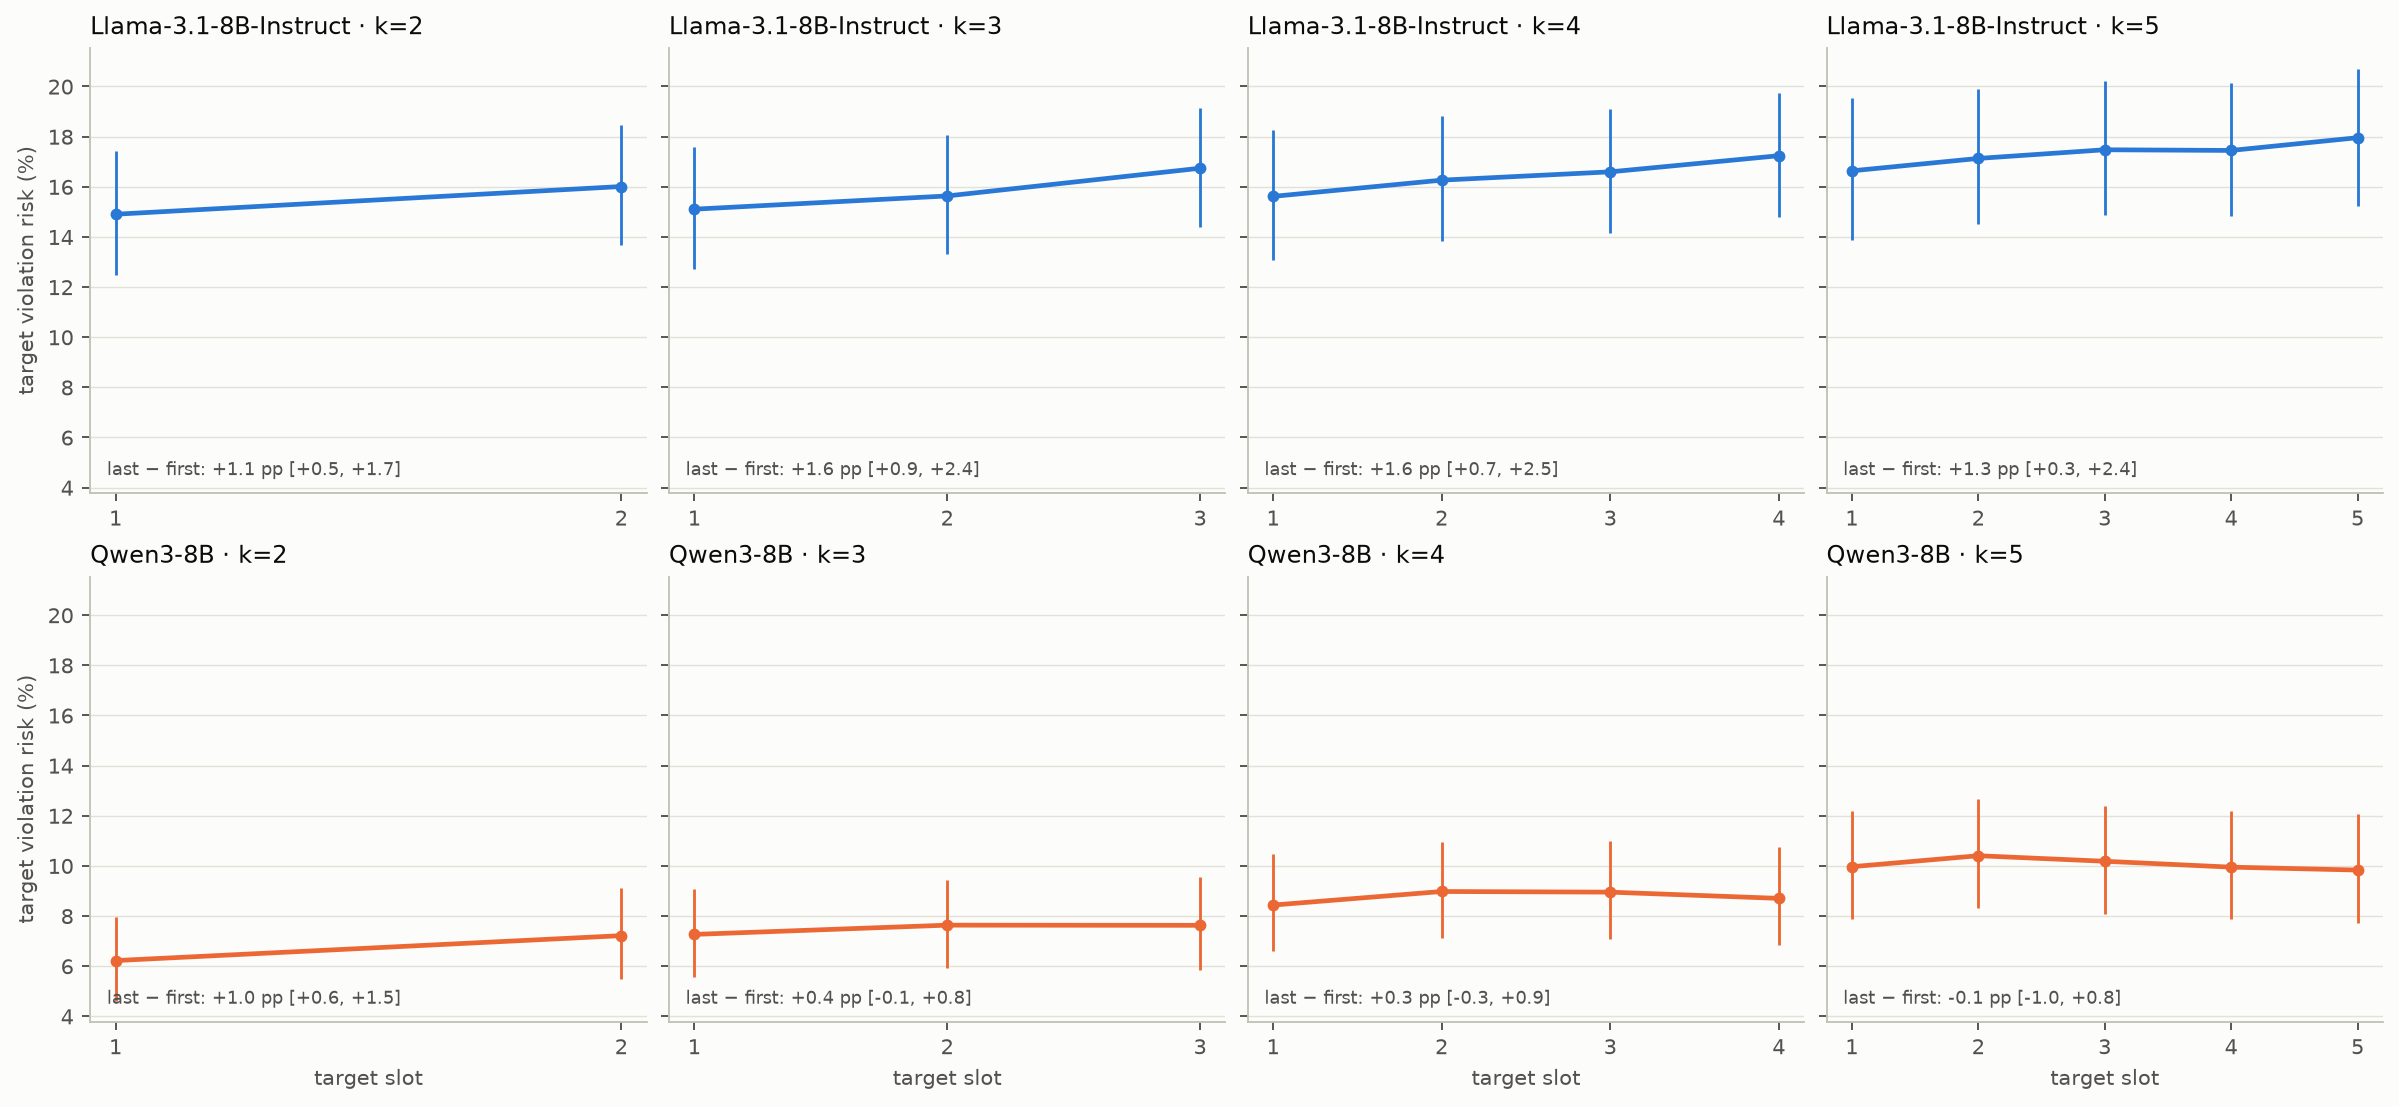
\includegraphics[width=\linewidth]{figures/prelim/e2_posA_slot_curves.png}\caption{Pos-A. Observed violation risk at every slot, by $k$ (COA-balanced, 95\% pool intervals).}\end{figure}
\begin{table}[h]
\centering\scriptsize
\caption{Pos-A. Signed change (later slot $-$ earlier slot, points) for all 20 position-pair strata, 50 pools.}
\label{tab:posA}
\begin{tabular}{ccccc}
\toprule
$k$ & Slots & Llama & Qwen & Contexts \\
\midrule
2 & 1$\to$2 & 1.11 [0.48, 1.71] & 0.99 [0.57, 1.45] & 1800 \\
3 & 1$\to$2 & 0.53 [$-$0.02, 1.06] & 0.37 [0.05, 0.71] & 2700 \\
3 & 1$\to$3 & 1.63 [0.90, 2.36] & 0.36 [$-$0.06, 0.80] & 2700 \\
3 & 2$\to$3 & 1.11 [0.60, 1.62] & $-$0.01 [$-$0.34, 0.32] & 2700 \\
4 & 1$\to$2 & 0.65 [0.15, 1.12] & 0.54 [0.17, 0.95] & 3600 \\
4 & 1$\to$3 & 0.98 [0.31, 1.63] & 0.52 [0.03, 1.03] & 3600 \\
4 & 1$\to$4 & 1.62 [0.73, 2.52] & 0.27 [$-$0.30, 0.87] & 3600 \\
4 & 2$\to$3 & 0.33 [0.01, 0.66] & $-$0.03 [$-$0.27, 0.22] & 3600 \\
4 & 2$\to$4 & 0.98 [0.33, 1.64] & $-$0.27 [$-$0.64, 0.10] & 3600 \\
4 & 3$\to$4 & 0.64 [0.16, 1.12] & $-$0.25 [$-$0.51, 0.00] & 3600 \\
5 & 1$\to$2 & 0.50 [0.01, 0.97] & 0.44 [0.01, 0.91] & 4500 \\
5 & 1$\to$3 & 0.84 [0.13, 1.51] & 0.22 [$-$0.42, 0.90] & 4500 \\
5 & 1$\to$4 & 0.81 [$-$0.09, 1.66] & $-$0.02 [$-$0.76, 0.75] & 4500 \\
5 & 1$\to$5 & 1.32 [0.25, 2.39] & $-$0.13 [$-$1.01, 0.76] & 4500 \\
5 & 2$\to$3 & 0.35 [0.05, 0.64] & $-$0.22 [$-$0.56, 0.16] & 4500 \\
5 & 2$\to$4 & 0.32 [$-$0.20, 0.84] & $-$0.46 [$-$0.97, 0.07] & 4500 \\
5 & 2$\to$5 & 0.83 [0.05, 1.62] & $-$0.57 [$-$1.24, 0.08] & 4500 \\
5 & 3$\to$4 & $-$0.03 [$-$0.32, 0.28] & $-$0.23 [$-$0.53, 0.08] & 4500 \\
5 & 3$\to$5 & 0.48 [$-$0.17, 1.12] & $-$0.35 [$-$0.79, 0.06] & 4500 \\
5 & 4$\to$5 & 0.51 [0.04, 0.95] & $-$0.12 [$-$0.35, 0.11] & 4500 \\
\bottomrule
\end{tabular}
\end{table}

\subsection*{Pos-B --- Predicting position changes by $k$}
\begin{table}[h]
\centering\scriptsize
\caption{Pos-B. Paired $\Delta$-MSE reduction ($\times10^4$) [95\% interval] by $k$; positive favours the candidate. $\Delta$-MAE: \texttt{tables/eval2\_position\_skill.csv}.}
\label{tab:Pos-B}
\resizebox{\linewidth}{!}{
\begin{tabular}{llcccc}
\toprule
 & Comparison & $k$ 2 & $k$ 3 & $k$ 4 & $k$ 5 \\
\midrule
Llama & 1: B1 \cto{} H1 & 2.0 [$-$10.4, 14.9] & 1.0 [$-$4.4, 6.6] & 2.2 [$-$1.8, 6.2] & 2.8 [$-$1.1, 7.1] \\
 & 2: B2 \cto{} H2 & 10.9 [2.0, 21.4] & 6.0 [1.9, 10.5] & 4.0 [0.7, 7.5] & 3.6 [0.2, 7.3] \\
 & 3: B2 \cto{} RCAP & $-$77.1 [$-$118.3, $-$40.3] & $-$36.2 [$-$55.7, $-$19.4] & $-$23.8 [$-$36.7, $-$12.1] & $-$12.1 [$-$21.5, $-$3.0] \\
 & 4: H2 \cto{} RCAP & $-$88.0 [$-$127.1, $-$53.6] & $-$42.2 [$-$60.4, $-$26.9] & $-$27.8 [$-$39.5, $-$17.0] & $-$15.7 [$-$24.3, $-$7.5] \\
 & 5: B1 \cto{} B1+H1 & $-$2.9 [$-$19.1, 13.9] & 0.1 [$-$7.1, 7.8] & 2.6 [$-$3.4, 8.7] & 4.6 [$-$1.4, 10.9] \\
 & 6: B2 \cto{} B2+H1 & 11.0 [2.7, 20.9] & 6.9 [2.4, 11.8] & 4.9 [1.4, 8.6] & 4.6 [1.4, 8.2] \\
 & 7: B2 \cto{} B2+A1 & $-$42.6 [$-$68.6, $-$18.2] & $-$15.5 [$-$29.9, $-$2.6] & $-$7.7 [$-$16.6, 0.6] & $-$0.1 [$-$7.0, 7.0] \\
 & zero-change MSE & 181.3 & 140.2 & 117.6 & 110.5 \\
\midrule
Qwen & 1: B1 \cto{} H1 & $-$14.8 [$-$31.4, $-$5.2] & $-$6.9 [$-$11.7, $-$3.0] & $-$2.6 [$-$5.1, $-$0.3] & $-$0.4 [$-$3.6, 2.7] \\
 & 2: B2 \cto{} H2 & $-$13.4 [$-$27.4, $-$5.1] & $-$5.9 [$-$10.1, $-$2.5] & $-$1.7 [$-$3.9, 0.3] & $-$0.3 [$-$3.1, 2.4] \\
 & 3: B2 \cto{} RCAP & $-$23.6 [$-$38.6, $-$9.0] & $-$19.3 [$-$27.3, $-$12.1] & $-$18.9 [$-$25.5, $-$13.1] & $-$13.4 [$-$19.7, $-$8.0] \\
 & 4: H2 \cto{} RCAP & $-$10.2 [$-$26.6, 7.3] & $-$13.4 [$-$21.2, $-$6.0] & $-$17.2 [$-$23.7, $-$11.4] & $-$13.1 [$-$19.2, $-$7.6] \\
 & 5: B1 \cto{} B1+H1 & $-$11.6 [$-$24.0, $-$4.1] & $-$3.9 [$-$6.7, $-$1.5] & $-$0.7 [$-$2.6, 1.0] & 0.6 [$-$1.9, 3.2] \\
 & 6: B2 \cto{} B2+H1 & $-$13.0 [$-$26.6, $-$4.9] & $-$5.5 [$-$9.5, $-$2.3] & $-$1.4 [$-$3.6, 0.5] & $-$0.2 [$-$2.9, 2.5] \\
 & 7: B2 \cto{} B2+A1 & $-$22.2 [$-$36.5, $-$8.3] & $-$17.8 [$-$25.4, $-$11.0] & $-$17.4 [$-$23.4, $-$12.0] & $-$12.1 [$-$18.1, $-$7.1] \\
 & zero-change MSE & 105.1 & 84.9 & 77.0 & 81.0 \\
\bottomrule
\end{tabular}
}
\end{table}

\subsection*{Pos-C --- Numerical position estimates and noise diagnostics}
\begin{table}[h]
\centering\scriptsize
\caption{Pos-C. Position: corrected and raw squared changes, binomial noise floor ($\times10^4$), baseline risk and support by target type. Signed type $\times k$ values with intervals: \texttt{tables/eval2\_position\_signed\_type\_k.csv}.}
\label{tab:posC}
\resizebox{\linewidth}{!}{
\begin{tabular}{lcccccccccc}
\toprule
Type & L RMS & L corr. & L noise & L base & L pools & Q RMS & Q corr. & Q noise & Q base & Q pools \\
\midrule
\texttt{english\_capital} & 5.1 [3.2, 6.6] & 26.0 & 49.4 & 14.4 & 18 & 6.8 [5.4, 8.2] & 46.8 & 36.4 & 14.6 & 18 \\
\texttt{english\_lowercase} & 0.0 [0.0, 0.9] & $-$0.8 & 13.3 & 2.2 & 10 & 1.1 [0.4, 1.6] & 1.2 & 4.1 & 0.8 & 10 \\
\texttt{title} & 12.7 [6.5, 17.6] & 161.9 & 2.9 & 3.2 & 26 & 0.7 [0.0, 1.3] & 0.5 & 0.2 & 0.0 & 26 \\
\texttt{no\_comma} & 7.5 [5.4, 9.3] & 55.7 & 19.4 & 6.9 & 27 & 4.4 [0.2, 8.1] & 19.7 & 0.2 & 0.1 & 27 \\
\texttt{quotation} & 11.1 [8.2, 13.7] & 122.8 & 38.3 & 19.0 & 22 & 5.2 [3.7, 6.5] & 26.6 & 9.1 & 5.0 & 22 \\
\texttt{capital\_word\_frequency} & 9.8 [6.6, 12.6] & 95.3 & 42.5 & 27.3 & 12 & 13.3 [10.4, 16.0] & 175.8 & 27.0 & 27.1 & 12 \\
\texttt{number\_placeholders} & 9.6 [7.4, 11.5] & 92.1 & 45.7 & 21.7 & 27 & 6.7 [5.0, 8.1] & 44.2 & 13.4 & 6.4 & 27 \\
\texttt{number\_bullet\_lists} & 16.7 [14.5, 19.0] & 280.0 & 52.1 & 28.2 & 25 & 20.9 [17.2, 24.2] & 435.6 & 16.4 & 15.3 & 25 \\
\texttt{existence} & 5.2 [3.6, 6.4] & 26.8 & 31.1 & 8.7 & 15 & 4.1 [2.5, 5.5] & 16.6 & 12.5 & 4.6 & 15 \\
\texttt{forbidden\_words} & 0.0 [0.0, 1.0] & $-$1.4 & 9.2 & 1.8 & 29 & 1.9 [0.8, 2.8] & 3.6 & 8.8 & 2.2 & 29 \\
\texttt{frequency} & 5.3 [2.9, 7.7] & 28.1 & 16.6 & 4.6 & 18 & 4.0 [2.2, 5.7] & 16.0 & 7.1 & 2.5 & 18 \\
\texttt{letter\_frequency} & 6.0 [2.3, 9.0] & 35.8 & 11.5 & 34.9 & 29 & 6.5 [3.2, 9.7] & 42.0 & 9.8 & 31.7 & 29 \\
\texttt{number\_paragraphs} & 24.4 [21.9, 26.6] & 595.5 & 70.8 & 50.4 & 17 & 7.5 [4.0, 10.5] & 55.7 & 5.5 & 5.0 & 17 \\
\texttt{number\_sentences} & 7.8 [3.7, 11.0] & 61.3 & 35.0 & 19.6 & 11 & 12.2 [7.2, 16.1] & 148.8 & 15.1 & 10.8 & 11 \\
\texttt{number\_words} & 5.0 [3.1, 6.6] & 25.1 & 14.3 & 9.2 & 14 & 11.9 [7.8, 15.3] & 141.6 & 27.5 & 17.1 & 14 \\
\bottomrule
\end{tabular}
}
\end{table}

\subsection*{K-A --- Observed append effect by retained slot and transition}
\begin{table}[h]
\centering\scriptsize
\caption{K-A. Mean change in retained-rule violation risk (points) by transition and retained slot; the new rule is excluded. 1$\to$2 and 2$\to$3 cover every chain prefix; 3$\to$4 and 4$\to$5 only COA orders with an exact prefix.}
\label{tab:KA}
\begin{tabular}{ccccc}
\toprule
Transition & Slot & Llama & Qwen & Targets \\
\midrule
1$\to$2 & 1 & $-$0.52 [$-$1.68, 0.65] & 0.37 [$-$0.32, 1.06] & 1,800 \\
2$\to$3 & 1 & 0.30 [$-$0.35, 0.93] & 1.10 [0.38, 1.91] & 3,600 \\
2$\to$3 & 2 & $-$0.36 [$-$1.11, 0.37] & 0.55 [$-$0.11, 1.26] & 3,600 \\
3$\to$4 & 1 & 0.56 [$-$0.19, 1.34] & 1.12 [0.50, 1.74] & 5,400 \\
3$\to$4 & 2 & 0.69 [0.03, 1.40] & 1.41 [0.73, 2.12] & 5,400 \\
3$\to$4 & 3 & 0.08 [$-$0.62, 0.82] & 1.18 [0.62, 1.77] & 5,400 \\
4$\to$5 & 1 & 1.38 [0.65, 2.11] & 1.59 [0.95, 2.27] & 3,600 \\
4$\to$5 & 2 & 0.89 [0.12, 1.77] & 1.40 [0.66, 2.28] & 3,600 \\
4$\to$5 & 3 & 0.50 [$-$0.28, 1.35] & 1.49 [0.89, 2.13] & 3,600 \\
4$\to$5 & 4 & 0.12 [$-$0.54, 0.81] & 1.06 [0.51, 1.67] & 3,600 \\
\bottomrule
\end{tabular}
\end{table}

\subsection*{K-B --- Predicting append changes by transition}
\begin{table}[h]
\centering\scriptsize
\caption{K-B. Paired $\Delta$-MSE reduction ($\times10^4$) [95\% interval] by transition; positive favours the candidate. $\Delta$-MAE: \texttt{tables/eval2\_append\_skill.csv}.}
\label{tab:K-B}
\resizebox{\linewidth}{!}{
\begin{tabular}{llcccc}
\toprule
 & Comparison & transition 1$\to$2 & transition 2$\to$3 & transition 3$\to$4 & transition 4$\to$5 \\
\midrule
Llama & 1: B1 \cto{} H1 & $-$44.0 [$-$87.6, $-$8.4] & $-$20.6 [$-$46.3, 1.7] & $-$12.2 [$-$26.3, 0.2] & $-$11.0 [$-$24.2, 0.2] \\
 & 2: B2 \cto{} H2 & $-$1.2 [$-$13.5, 10.8] & 4.2 [$-$5.5, 13.7] & 4.9 [$-$0.2, 10.0] & 3.6 [$-$0.7, 8.1] \\
 & 3: B2 \cto{} RCAP & $-$30.2 [$-$64.2, 3.2] & $-$26.5 [$-$46.8, $-$7.6] & $-$20.1 [$-$31.0, $-$10.4] & $-$12.2 [$-$22.4, $-$2.8] \\
 & 4: H2 \cto{} RCAP & $-$29.0 [$-$62.3, 3.6] & $-$30.7 [$-$46.1, $-$16.5] & $-$25.0 [$-$36.8, $-$14.5] & $-$15.8 [$-$27.4, $-$5.8] \\
 & 5: B1 \cto{} B1+H1 & $-$57.0 [$-$97.3, $-$21.2] & $-$9.9 [$-$34.4, 12.8] & $-$3.7 [$-$16.9, 8.9] & $-$0.2 [$-$12.6, 11.2] \\
 & 6: B2 \cto{} B2+H1 & 5.9 [$-$5.6, 17.3] & 9.8 [1.3, 18.6] & 8.8 [4.5, 13.1] & 7.7 [4.3, 11.4] \\
 & 7: B2 \cto{} B2+A1 & $-$1.6 [$-$28.4, 25.9] & $-$2.6 [$-$18.1, 12.0] & 0.8 [$-$5.5, 7.2] & 5.2 [$-$1.7, 12.7] \\
 & zero-change MSE & 263.1 & 227.5 & 238.8 & 211.9 \\
\midrule
Qwen & 1: B1 \cto{} H1 & $-$23.5 [$-$49.2, $-$1.9] & $-$21.0 [$-$40.8, $-$3.3] & $-$13.0 [$-$22.7, $-$4.3] & $-$9.1 [$-$18.4, $-$0.5] \\
 & 2: B2 \cto{} H2 & $-$10.2 [$-$25.2, 4.2] & $-$10.7 [$-$21.8, $-$0.6] & $-$2.7 [$-$10.0, 4.6] & 3.3 [$-$5.2, 12.5] \\
 & 3: B2 \cto{} RCAP & $-$14.5 [$-$33.4, 4.0] & $-$12.5 [$-$23.6, $-$2.5] & $-$9.2 [$-$19.1, 1.1] & $-$13.2 [$-$23.8, $-$3.1] \\
 & 4: H2 \cto{} RCAP & $-$4.3 [$-$22.3, 13.3] & $-$1.8 [$-$11.0, 8.0] & $-$6.5 [$-$13.5, 0.5] & $-$16.5 [$-$26.8, $-$7.9] \\
 & 5: B1 \cto{} B1+H1 & $-$16.3 [$-$35.5, 0.3] & $-$13.9 [$-$28.4, $-$1.4] & $-$5.4 [$-$12.4, 0.9] & $-$0.3 [$-$6.6, 5.8] \\
 & 6: B2 \cto{} B2+H1 & $-$9.4 [$-$23.9, 4.9] & $-$9.9 [$-$20.5, $-$0.3] & $-$1.5 [$-$8.7, 5.7] & 4.7 [$-$3.5, 13.8] \\
 & 7: B2 \cto{} B2+A1 & $-$13.2 [$-$31.1, 4.6] & $-$10.8 [$-$21.4, $-$1.1] & $-$7.4 [$-$17.0, 2.8] & $-$10.9 [$-$21.2, $-$1.1] \\
 & zero-change MSE & 163.5 & 167.1 & 199.7 & 192.4 \\
\bottomrule
\end{tabular}
}
\end{table}

\subsection*{C-A --- Companion effects by $k$ and placement; numerical support}
\begin{table}[h]
\centering\scriptsize
\caption{C-A. Noise-adjusted RMS companion-replacement sensitivity (points) by $k$ and whether the replaced companion is earlier or later than the target. Signed target $\times$ companion cells with intervals and support: \texttt{tables/eval2\_companion\_signed\_matrix.csv}.}
\label{tab:CA}
\begin{tabular}{ccccc}
\toprule
$k$ & Companion & Llama & Qwen & Comparisons \\
\midrule
2 & earlier & 18.4 [15.8, 21.0] & 15.4 [12.6, 18.0] & 900 \\
2 & later & 16.3 [13.7, 19.1] & 12.7 [10.2, 15.1] & 900 \\
2 & both & 17.4 [15.0, 19.9] & 14.1 [11.8, 16.4] & 1,800 \\
3 & earlier & 17.2 [15.4, 18.8] & 15.9 [13.8, 18.0] & 5,400 \\
3 & later & 15.1 [13.3, 17.0] & 14.3 [11.9, 16.6] & 5,400 \\
3 & both & 16.2 [14.5, 17.8] & 15.1 [13.0, 17.2] & 10,800 \\
5 & earlier & 16.0 [14.3, 17.7] & 17.4 [15.0, 19.8] & 36,000 \\
5 & later & 15.1 [13.3, 17.1] & 16.4 [14.4, 18.3] & 36,000 \\
5 & both & 15.6 [13.9, 17.4] & 16.9 [14.8, 19.0] & 72,000 \\
macro & earlier & 17.2 [15.5, 18.9] & 16.3 [14.3, 18.1] & 42,300 \\
macro & later & 15.5 [13.8, 17.3] & 14.5 [12.8, 16.2] & 42,300 \\
\bottomrule
\end{tabular}
\end{table}

\begin{table}[h]
\centering\scriptsize
\caption{C-A (by target type). Corrected and raw squared changes, binomial noise floor ($\times10^4$), baseline risk and support.}
\label{tab:CAt}
\resizebox{\linewidth}{!}{
\begin{tabular}{lcccccccccc}
\toprule
Type & L RMS & L corr. & L noise & L base & L pools & Q RMS & Q corr. & Q noise & Q base & Q pools \\
\midrule
\texttt{english\_capital} & 10.4 [7.4, 13.0] & 107.5 & 94.4 & 14.4 & 18 & 21.1 [14.8, 27.7] & 443.3 & 71.3 & 15.0 & 18 \\
\texttt{english\_lowercase} & 3.1 [1.6, 4.5] & 9.9 & 24.2 & 2.2 & 10 & 2.4 [1.2, 3.3] & 5.7 & 7.2 & 0.7 & 10 \\
\texttt{title} & 12.3 [6.3, 17.2] & 151.5 & 6.4 & 3.4 & 26 & 0.9 [0.0, 1.7] & 0.8 & 0.4 & 0.0 & 26 \\
\texttt{no\_comma} & 15.1 [9.7, 20.3] & 227.2 & 37.1 & 6.8 & 27 & 5.1 [0.3, 9.3] & 25.8 & 0.5 & 0.1 & 27 \\
\texttt{quotation} & 27.3 [20.3, 33.8] & 742.9 & 78.3 & 20.3 & 22 & 12.4 [7.1, 17.4] & 153.8 & 20.7 & 5.4 & 22 \\
\texttt{capital\_word\_frequency} & 18.0 [13.1, 21.9] & 322.3 & 80.3 & 26.8 & 12 & 32.9 [23.5, 41.5] & 1081.4 & 52.4 & 27.1 & 12 \\
\texttt{number\_placeholders} & 12.9 [10.8, 14.9] & 167.0 & 92.5 & 22.7 & 27 & 10.5 [7.6, 13.2] & 110.4 & 29.0 & 6.9 & 27 \\
\texttt{number\_bullet\_lists} & 23.8 [20.8, 26.5] & 568.6 & 103.8 & 28.3 & 25 & 27.4 [23.7, 30.8] & 751.8 & 37.6 & 16.7 & 25 \\
\texttt{existence} & 11.3 [7.0, 15.3] & 128.3 & 59.7 & 8.6 & 15 & 11.6 [5.6, 17.7] & 134.4 & 26.4 & 4.8 & 15 \\
\texttt{forbidden\_words} & 3.4 [1.3, 5.3] & 11.7 & 17.5 & 1.8 & 29 & 6.4 [2.5, 9.9] & 41.0 & 17.2 & 2.3 & 29 \\
\texttt{frequency} & 7.7 [4.5, 10.6] & 59.9 & 32.6 & 4.6 & 18 & 6.6 [3.9, 8.8] & 44.1 & 14.0 & 2.4 & 18 \\
\texttt{letter\_frequency} & 9.0 [5.0, 12.4] & 81.5 & 23.0 & 35.0 & 29 & 12.6 [8.1, 16.4] & 158.2 & 18.6 & 31.6 & 29 \\
\texttt{number\_paragraphs} & 31.8 [27.6, 35.7] & 1009.0 & 133.1 & 50.8 & 17 & 13.1 [6.5, 18.4] & 171.7 & 13.0 & 5.3 & 17 \\
\texttt{number\_sentences} & 19.9 [12.9, 25.4] & 397.8 & 67.1 & 19.7 & 11 & 25.7 [16.6, 32.4] & 659.5 & 29.4 & 11.2 & 11 \\
\texttt{number\_words} & 12.9 [5.4, 19.0] & 167.3 & 33.2 & 10.3 & 14 & 20.3 [14.6, 24.9] & 411.1 & 59.4 & 18.3 & 14 \\
\bottomrule
\end{tabular}
}
\end{table}

\subsection*{C-B --- Predicting companion changes by $k$}
\begin{table}[h]
\centering\scriptsize
\caption{C-B. Paired $\Delta$-MSE reduction ($\times10^4$) [95\% interval] by $k$; positive favours the candidate. $\Delta$-MAE: \texttt{tables/eval2\_companion\_skill.csv}.}
\label{tab:C-B}
\resizebox{\linewidth}{!}{
\begin{tabular}{llccc}
\toprule
 & Comparison & $k$ 2 & $k$ 3 & $k$ 5 \\
\midrule
Llama & 1: B1 \cto{} H1 & $-$68.7 [$-$132.3, $-$15.2] & $-$27.8 [$-$65.4, 4.0] & $-$16.1 [$-$34.0, 0.1] \\
 & 2: B2 \cto{} H2 & 16.3 [$-$3.3, 36.6] & 1.4 [$-$10.9, 13.2] & 7.0 [$-$1.4, 15.3] \\
 & 3: B2 \cto{} RCAP & $-$23.0 [$-$58.1, 14.5] & $-$27.5 [$-$48.5, $-$7.8] & $-$7.7 [$-$19.4, 4.3] \\
 & 4: H2 \cto{} RCAP & $-$39.3 [$-$75.2, $-$3.4] & $-$28.9 [$-$50.9, $-$6.6] & $-$14.7 [$-$30.8, 1.3] \\
 & 5: B1 \cto{} B1+H1 & $-$73.8 [$-$145.4, $-$15.0] & $-$22.8 [$-$57.3, 9.0] & 0.5 [$-$15.9, 16.8] \\
 & 6: B2 \cto{} B2+H1 & 22.8 [8.2, 37.8] & 9.9 [$-$0.9, 20.0] & 14.2 [7.3, 21.2] \\
 & 7: B2 \cto{} B2+A1 & 9.9 [$-$16.6, 41.3] & $-$1.6 [$-$13.6, 9.6] & 12.5 [3.3, 22.4] \\
 & zero-change MSE & 355.2 & 318.0 & 303.1 \\
\midrule
Qwen & 1: B1 \cto{} H1 & $-$76.9 [$-$146.1, $-$22.6] & $-$26.3 [$-$54.5, $-$0.6] & 1.4 [$-$14.9, 18.4] \\
 & 2: B2 \cto{} H2 & $-$46.2 [$-$85.5, $-$13.1] & $-$15.3 [$-$32.8, 1.7] & 18.4 [0.3, 41.9] \\
 & 3: B2 \cto{} RCAP & 4.2 [$-$23.2, 33.3] & $-$27.9 [$-$50.3, $-$7.7] & 5.7 [$-$12.1, 25.1] \\
 & 4: H2 \cto{} RCAP & 50.5 [7.8, 99.5] & $-$12.6 [$-$31.2, 6.6] & $-$12.7 [$-$29.1, 2.4] \\
 & 5: B1 \cto{} B1+H1 & $-$58.6 [$-$107.8, $-$18.3] & $-$15.6 [$-$35.2, 2.2] & 11.0 [$-$1.4, 25.4] \\
 & 6: B2 \cto{} B2+H1 & $-$44.5 [$-$82.1, $-$12.6] & $-$14.0 [$-$31.0, 2.6] & 19.8 [1.8, 43.4] \\
 & 7: B2 \cto{} B2+A1 & 5.7 [$-$22.3, 35.3] & $-$25.6 [$-$47.4, $-$6.0] & 8.4 [$-$9.6, 27.9] \\
 & zero-change MSE & 218.4 & 252.1 & 316.1 \\
\bottomrule
\end{tabular}
}
\end{table}

\subsection*{D-A --- Task sensitivity by target type and $k$}
\begin{table}[h]
\centering\scriptsize
\caption{D-A. Noise-adjusted RMS task sensitivity (points) by type and $k$ (intervals in \texttt{tables/eval2\_task\_rms\_type\_k.csv}).}
\label{tab:DA}
\resizebox{\linewidth}{!}{
\begin{tabular}{lcccccccccc}
\toprule
Type & L $k{=}1$ & L $k{=}2$ & L $k{=}3$ & L $k{=}4$ & L $k{=}5$ & Q $k{=}1$ & Q $k{=}2$ & Q $k{=}3$ & Q $k{=}4$ & Q $k{=}5$ \\
\midrule
\texttt{english\_capital} & 29.2 & 28.5 & 24.9 & 24.8 & 24.9 & 25.8 & 28.2 & 28.0 & 28.2 & 29.0 \\
\texttt{english\_lowercase} & 14.7 & 7.7 & 6.1 & 6.3 & 6.0 & 4.6 & 2.5 & 1.6 & 3.4 & 3.6 \\
\texttt{title} & 0.0 & 7.1 & 11.9 & 13.1 & 15.0 & 0.0 & 1.0 & 1.1 & 1.7 & 0.8 \\
\texttt{no\_comma} & 24.8 & 19.6 & 22.9 & 22.1 & 21.8 & 15.8 & 7.9 & 3.8 & 1.8 & 2.8 \\
\texttt{quotation} & 13.5 & 25.2 & 22.7 & 20.9 & 21.4 & 1.3 & 7.9 & 9.8 & 12.8 & 14.0 \\
\texttt{capital\_word\_frequency} & 39.7 & 43.8 & 43.4 & 42.6 & 40.7 & 52.6 & 52.4 & 48.2 & 48.1 & 49.7 \\
\texttt{number\_placeholders} & 27.1 & 27.3 & 28.1 & 27.7 & 29.2 & 6.2 & 9.9 & 14.3 & 17.3 & 19.5 \\
\texttt{number\_bullet\_lists} & 61.6 & 49.9 & 45.1 & 42.0 & 40.2 & 19.4 & 24.6 & 27.3 & 28.1 & 30.5 \\
\texttt{existence} & 19.9 & 16.2 & 18.0 & 18.3 & 18.5 & 1.5 & 13.9 & 10.3 & 12.6 & 14.1 \\
\texttt{forbidden\_words} & 5.8 & 7.1 & 7.8 & 5.6 & 5.7 & 10.3 & 6.9 & 8.7 & 8.4 & 6.9 \\
\texttt{frequency} & 16.2 & 14.4 & 12.5 & 12.0 & 11.5 & 11.1 & 14.0 & 12.1 & 12.5 & 11.3 \\
\texttt{letter\_frequency} & 21.6 & 18.9 & 18.9 & 19.3 & 18.6 & 24.9 & 20.9 & 21.5 & 21.7 & 20.5 \\
\texttt{number\_paragraphs} & 50.0 & 41.0 & 38.6 & 36.3 & 34.9 & 5.0 & 2.5 & 11.1 & 13.8 & 14.9 \\
\texttt{number\_sentences} & 40.1 & 36.4 & 36.7 & 38.9 & 40.6 & 17.4 & 29.9 & 21.0 & 24.6 & 30.4 \\
\texttt{number\_words} & 1.6 & 8.5 & 13.7 & 19.0 & 21.0 & 4.2 & 12.3 & 22.9 & 24.5 & 24.3 \\
\bottomrule
\end{tabular}
}
\end{table}

\subsection*{D-B --- Rule type $\times$ task family}
\begin{figure}[h]\centering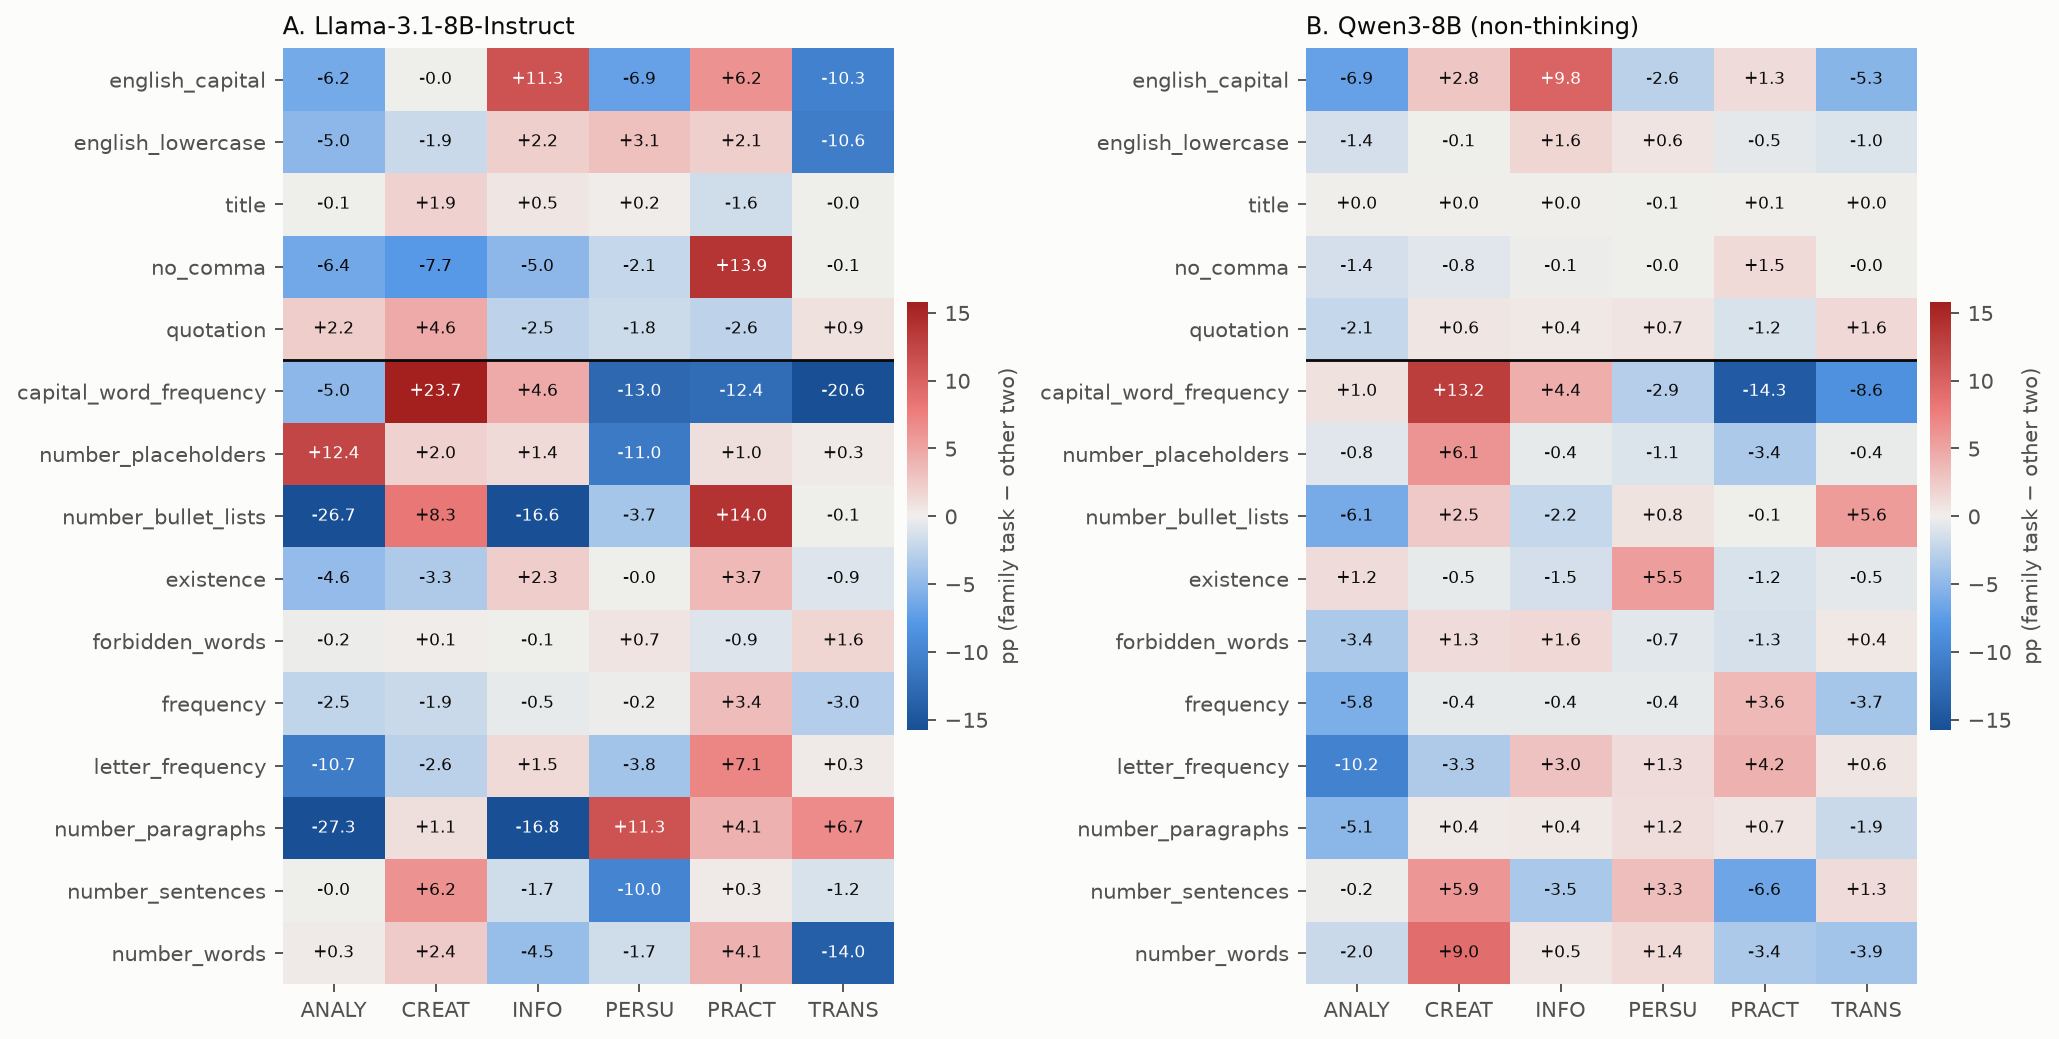
\includegraphics[width=\linewidth]{figures/prelim/e2_taskDB_type_family_heatmap.png}\caption{D-B. Signed family-task minus mean of the other two matched tasks (points), by target type and family. Descriptive associations; family is confounded with task text.}\end{figure}
\subsection*{D-C --- Predicting task changes by $k$}
\begin{table}[h]
\centering\scriptsize
\caption{D-C. Paired $\Delta$-MSE reduction ($\times10^4$) [95\% interval] by $k$; positive favours the candidate. $\Delta$-MAE: \texttt{tables/eval2\_task\_skill.csv}.}
\label{tab:D-C}
\resizebox{\linewidth}{!}{
\begin{tabular}{llccccc}
\toprule
 & Comparison & $k$ 1 & $k$ 2 & $k$ 3 & $k$ 4 & $k$ 5 \\
\midrule
Llama & 1: B1 \cto{} H1 & 214.2 [89.4, 345.5] & 144.0 [45.9, 245.8] & 148.5 [69.5, 231.8] & 150.9 [77.6, 229.9] & 151.3 [82.1, 228.0] \\
 & 2: B2 \cto{} H2 & 202.6 [76.9, 338.7] & 119.1 [20.1, 220.0] & 111.5 [38.2, 186.6] & 105.4 [42.1, 172.2] & 96.9 [43.1, 154.9] \\
 & 3: B2 \cto{} RCAP & 83.4 [$-$79.2, 247.9] & 11.4 [$-$89.7, 110.0] & 53.1 [$-$14.8, 122.9] & 64.2 [11.3, 122.1] & 74.7 [30.0, 125.3] \\
 & 4: H2 \cto{} RCAP & $-$119.3 [$-$207.9, $-$34.8] & $-$107.7 [$-$165.2, $-$56.6] & $-$58.5 [$-$92.1, $-$25.9] & $-$41.1 [$-$68.9, $-$12.9] & $-$22.3 [$-$47.6, 3.1] \\
 & 5: B1 \cto{} B1+H1 & 137.5 [$-$9.9, 288.6] & 111.5 [$-$0.5, 224.2] & 111.5 [16.6, 206.5] & 106.3 [16.2, 199.2] & 97.1 [12.2, 184.5] \\
 & 6: B2 \cto{} B2+H1 & 171.0 [75.5, 275.7] & 114.2 [34.3, 195.8] & 104.0 [44.2, 164.3] & 96.2 [43.5, 150.2] & 84.7 [38.8, 131.1] \\
 & 7: B2 \cto{} B2+A1 & 115.5 [$-$9.3, 247.5] & 56.5 [$-$24.0, 137.7] & 67.1 [11.7, 125.1] & 64.7 [23.1, 109.3] & 63.0 [28.6, 100.7] \\
 & zero-change MSE & 904.9 & 753.5 & 715.3 & 686.9 & 683.3 \\
\midrule
Qwen & 1: B1 \cto{} H1 & $-$4.1 [$-$69.4, 57.7] & 16.7 [$-$29.8, 63.2] & 23.7 [$-$19.4, 70.1] & 39.9 [1.0, 82.7] & 39.2 [5.2, 78.1] \\
 & 2: B2 \cto{} H2 & $-$22.4 [$-$66.8, 25.4] & $-$39.8 [$-$66.1, $-$15.8] & $-$39.5 [$-$66.9, $-$14.2] & $-$26.0 [$-$48.0, $-$4.7] & $-$25.3 [$-$45.5, $-$6.0] \\
 & 3: B2 \cto{} RCAP & 7.3 [$-$54.2, 71.7] & $-$15.7 [$-$50.2, 16.5] & $-$32.6 [$-$57.0, $-$10.4] & $-$27.7 [$-$51.7, $-$5.7] & $-$23.8 [$-$45.9, $-$3.1] \\
 & 4: H2 \cto{} RCAP & 29.7 [$-$20.9, 89.1] & 24.1 [$-$3.7, 54.8] & 6.9 [$-$18.7, 31.1] & $-$1.7 [$-$24.6, 19.1] & 1.6 [$-$23.5, 25.3] \\
 & 5: B1 \cto{} B1+H1 & $-$11.5 [$-$63.8, 38.7] & 11.9 [$-$28.8, 56.4] & 22.4 [$-$19.8, 67.7] & 31.9 [$-$6.6, 75.6] & 29.7 [$-$4.2, 69.4] \\
 & 6: B2 \cto{} B2+H1 & $-$22.9 [$-$65.0, 23.2] & $-$39.9 [$-$66.3, $-$15.8] & $-$38.8 [$-$66.3, $-$13.6] & $-$25.8 [$-$47.9, $-$4.5] & $-$25.0 [$-$45.1, $-$5.9] \\
 & 7: B2 \cto{} B2+A1 & 8.0 [$-$52.0, 71.2] & $-$14.6 [$-$48.2, 16.8] & $-$29.9 [$-$52.9, $-$8.5] & $-$25.7 [$-$48.5, $-$4.8] & $-$21.8 [$-$43.1, $-$2.0] \\
 & zero-change MSE & 315.2 & 354.8 & 365.5 & 403.0 & 443.7 \\
\bottomrule
\end{tabular}
}
\end{table}

\subsection*{C-C and D-D --- Matching, weighting and validation}
Matched pairs are built from manifest metadata only. Companion: same pool, task, $k$, target rule and slot, every other slot identical, one companion differs, earlier and later replacements both included; the training design yields such pairs only at $k=2,3,5$. Task: each pool's 246 configurations appear with its three tasks (one per family), giving three unordered task pairs per target. Weights: equal per $k$ or transition, then pool, task, context and pair. The noise-adjusted RMS estimator and its 50-pool interval were checked by simulation (\texttt{tables/noise\_validation\_synthetic.csv}): mean estimate within 0.1 points of the true RMS whenever the true RMS is at least 3 points, an upward bias of 0.5--1 point at an exact null (truncation at zero), and 91--100\% coverage. Intervals are pointwise and unadjusted.

\begin{table}[h]
\centering\scriptsize
\caption{D-D. Task: corrected and raw squared changes, noise floor, baseline risk and support by target type.}
\label{tab:DD}
\resizebox{\linewidth}{!}{
\begin{tabular}{lcccccccccc}
\toprule
Type & L RMS & L corr. & L noise & L base & L pools & Q RMS & Q corr. & Q noise & Q base & Q pools \\
\midrule
\texttt{english\_capital} & 26.5 [17.6, 34.6] & 704.3 & 96.0 & 14.4 & 18 & 27.9 [21.3, 33.7] & 775.8 & 68.5 & 14.6 & 18 \\
\texttt{english\_lowercase} & 8.8 [3.7, 12.5] & 77.8 & 26.3 & 2.2 & 10 & 3.3 [1.5, 4.7] & 10.9 & 7.0 & 0.8 & 10 \\
\texttt{title} & 10.9 [5.0, 15.7] & 118.3 & 5.4 & 3.2 & 26 & 1.1 [0.0, 2.0] & 1.2 & 0.3 & 0.0 & 26 \\
\texttt{no\_comma} & 22.3 [16.4, 27.9] & 497.0 & 39.6 & 6.9 & 27 & 8.2 [0.4, 15.0] & 67.6 & 0.7 & 0.1 & 27 \\
\texttt{quotation} & 21.1 [15.6, 26.1] & 444.7 & 65.9 & 18.9 & 22 & 10.2 [6.9, 13.1] & 104.0 & 16.8 & 5.0 & 22 \\
\texttt{capital\_word\_frequency} & 42.1 [29.6, 52.1] & 1769.2 & 82.8 & 27.3 & 12 & 50.2 [39.7, 59.0] & 2523.5 & 57.9 & 27.1 & 12 \\
\texttt{number\_placeholders} & 27.9 [22.0, 33.4] & 778.1 & 90.4 & 21.7 & 27 & 14.3 [9.7, 18.8] & 204.4 & 27.0 & 6.4 & 27 \\
\texttt{number\_bullet\_lists} & 48.4 [42.6, 53.8] & 2338.8 & 98.3 & 28.2 & 25 & 26.3 [22.8, 29.4] & 689.6 & 32.1 & 15.2 & 25 \\
\texttt{existence} & 18.2 [11.9, 23.5] & 332.5 & 59.0 & 8.7 & 15 & 11.5 [6.9, 15.7] & 131.7 & 22.7 & 4.6 & 15 \\
\texttt{forbidden\_words} & 6.5 [3.2, 9.4] & 41.8 & 17.0 & 1.8 & 29 & 8.4 [4.1, 11.8] & 69.8 & 17.7 & 2.2 & 29 \\
\texttt{frequency} & 13.4 [6.9, 19.6] & 180.5 & 30.5 & 4.6 & 18 & 12.3 [4.4, 19.7] & 150.1 & 14.2 & 2.5 & 18 \\
\texttt{letter\_frequency} & 19.5 [8.0, 28.0] & 379.5 & 22.9 & 34.9 & 29 & 21.9 [13.4, 29.1] & 481.7 & 19.3 & 31.7 & 29 \\
\texttt{number\_paragraphs} & 40.5 [36.2, 44.7] & 1641.5 & 130.0 & 50.4 & 17 & 10.7 [6.2, 14.3] & 113.9 & 13.8 & 5.0 & 17 \\
\texttt{number\_sentences} & 38.6 [22.3, 51.4] & 1488.4 & 67.0 & 19.6 & 11 & 25.2 [15.9, 32.1] & 634.3 & 26.8 & 10.7 & 11 \\
\texttt{number\_words} & 14.6 [8.3, 19.6] & 213.6 & 27.5 & 9.1 & 14 & 19.4 [13.3, 25.2] & 376.2 & 49.7 & 17.0 & 14 \\
\bottomrule
\end{tabular}
}
\end{table}

\subsection*{Factor E --- Training-defined difficulty terciles}
\begin{table}[h]
\centering\scriptsize
\caption{Factor E. Types grouped by their $k=1$ training violation rate (5 per tercile); median noise-adjusted RMS (points) within tercile. On training data the terciles are defined on the data they stratify.}
\label{tab:E}
\begin{tabular}{llcccc}
\toprule
 & Tercile & $k{=}1$ rate (\%) & Position & Companion & Task \\
\midrule
Llama & easy & 0.0--3.7 & 5.3 & 12.3 & 13.4 \\
Llama & medium & 5.5--18.1 & 5.2 & 11.3 & 22.3 \\
Llama & hard & 21.7--47.0 & 9.8 & 19.9 & 40.5 \\
\midrule
Qwen & easy & 0.0--1.1 & 4.1 & 11.6 & 10.2 \\
Qwen & medium & 1.2--2.3 & 6.7 & 10.5 & 12.3 \\
Qwen & hard & 2.9--31.8 & 6.8 & 21.1 & 25.2 \\
\bottomrule
\end{tabular}
\end{table}

\subsection*{Evaluation 2, Objective 2 (preliminary design, not fixed by the plan)}
\begin{table}[h]
\centering\scriptsize
\caption{Objective~2 matched changes: prompt-level pairs, outcome = fraction of rules violated. Observed noise-adjusted RMS and signed mean (points; append includes the new rule, so the denominator changes); zero-change MSE and $\Delta$-MSE ($\times10^4$) for the primary comparisons. Secondary comparisons: \texttt{tables/obj2\_eval2.csv}.}
\label{tab:o2e2}
\resizebox{\linewidth}{!}{
\begin{tabular}{llcccccccc}
\toprule
 & Factor & Pairs & RMS & Signed mean & Zero MSE & 1 & 2 & 3 & 4 \\
\midrule
Llama & position & 244,800 & 6.9 [6.0, 7.7] & $-$0.08 [$-$0.35, 0.22] & 65.4 & $-$6.2 [$-$9.9, $-$2.3] & $-$3.7 [$-$5.9, $-$1.6] & $-$15.3 [$-$22.3, $-$8.9] & $-$11.6 [$-$17.3, $-$6.4] \\
 & append & 14,400 & 15.4 [14.1, 16.6] & 0.49 [$-$0.02, 1.01] & 259.8 & 57.8 [39.9, 76.4] & 16.1 [6.2, 26.8] & 14.4 [0.3, 28.8] & $-$1.7 [$-$15.3, 10.7] \\
 & companion & 25,200 & 16.7 [15.3, 18.1] & $-$0.22 [$-$1.12, 0.74] & 299.5 & 54.2 [29.6, 79.9] & 26.0 [14.4, 39.0] & 15.0 [$-$0.8, 32.7] & $-$11.0 [$-$24.7, 2.1] \\
 & task & 36,900 & 18.8 [16.9, 20.5] & $-$0.42 [$-$2.12, 1.22] & 376.3 & $-$3.1 [$-$42.1, 37.9] & 9.2 [$-$14.7, 34.1] & 13.5 [$-$28.3, 56.1] & 4.3 [$-$29.1, 35.0] \\
\midrule
Qwen & position & 244,800 & 6.1 [5.4, 6.8] & 0.06 [$-$0.07, 0.20] & 45.1 & $-$5.6 [$-$8.9, $-$2.8] & $-$5.6 [$-$8.7, $-$2.8] & $-$6.2 [$-$9.3, $-$3.6] & $-$0.6 [$-$2.6, 1.3] \\
 & append & 14,400 & 12.0 [10.5, 13.4] & 1.09 [0.72, 1.48] & 152.2 & 17.0 [8.6, 26.5] & 7.0 [$-$3.3, 17.2] & 9.8 [$-$0.4, 21.8] & 2.8 [$-$5.4, 11.1] \\
 & companion & 25,200 & 13.4 [11.7, 15.0] & 0.28 [$-$0.53, 1.17] & 188.0 & 20.7 [10.7, 32.2] & 12.7 [0.7, 25.6] & 6.5 [$-$4.3, 18.3] & $-$6.3 [$-$15.2, 1.9] \\
 & task & 36,900 & 12.6 [10.8, 14.2] & $-$0.44 [$-$1.67, 0.72] & 166.9 & $-$12.2 [$-$29.1, 2.9] & $-$11.8 [$-$28.9, 3.7] & $-$4.3 [$-$19.9, 12.2] & 7.5 [$-$3.8, 20.5] \\
\bottomrule
\end{tabular}
}
\end{table}

